\documentclass[11pt, a4paper]{ECON2123}
\usepackage{verbatim}
\usepackage{fancyhdr}
\usepackage{booktabs}
\usepackage{setspace}
\usepackage{amsmath,mathrsfs}
\usepackage{multicol}
\usepackage{amssymb}
\usepackage{graphicx}
\usepackage{caption}
\usepackage{subcaption}
\usepackage{array}
\usepackage{xcolor}
\usepackage{float}
\usepackage{enumitem}
\usepackage{mathcomp}
\usepackage{tabularx}
\usepackage{wasysym}
\usepackage{pbox}
\usepackage{tikz}
\usepackage{mathtools}
\usetikzlibrary{matrix}
\usepackage[normalem]{ulem}
\usepackage{multirow}
\usepackage[linesnumbered, ruled, boxed]{algorithm2e}
\SetKwRepeat{Do}{do}{while}

\title{Chapter 03}
\subtitle{The Goods Market}

\begin{document}
\begin{spacing}{1.5}

    \section{Overview of Goods Market}
    \begin{center}
        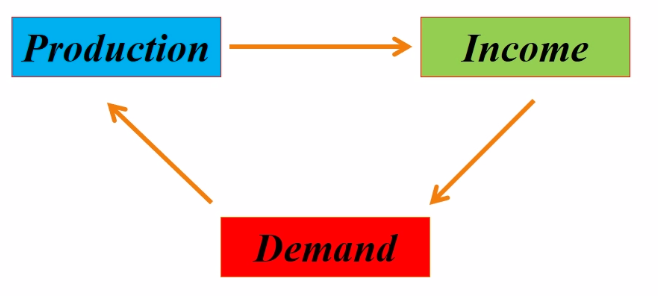
\includegraphics[scale=0.6]{images/03-overview.png}
    \end{center}
    \section{The Composition of GDP}

    Many purchases are very different decisions and depend on
    very different factors. So we want to understand the 
    demand for goods, we would like to decompose GDP from 
    the point of view of {\it different goods being produced},
    and {\it different buyers of these goods}.
    \begin{center}
        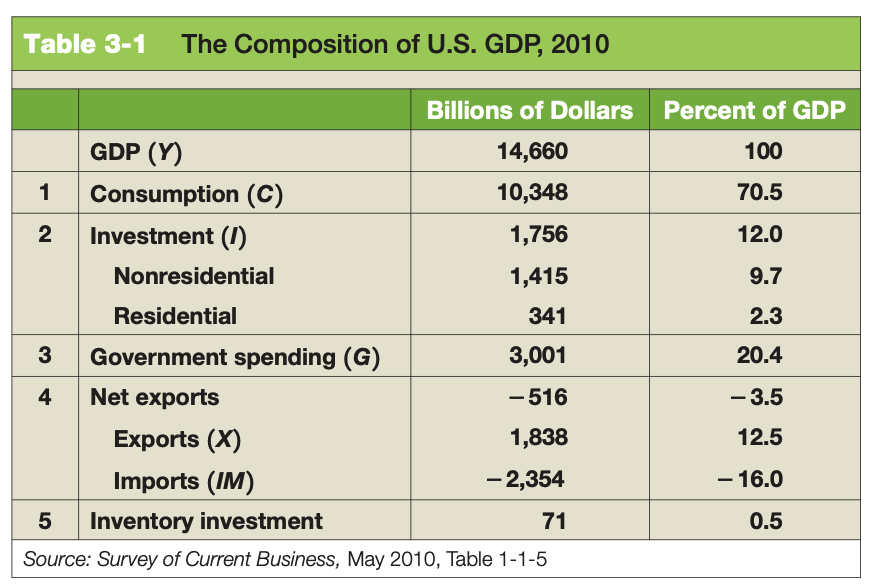
\includegraphics[scale=0.3]{images/03-composition-GDP.png}
    \end{center}
    \begin{itemize}
        \item {\bf consumption($C$):} goods and services purchased
        by consumers. The {\bf largest} component of GDP.
        \item {\bf (fixed) investment($I$):}  sum of 
        {\bf nonresidential investment} and {\bf residential investment}.
        In both cases, the decision to buy depends on the services 
        these goods will yield {\it in the future.} (notice this 
        difference from consumption)
        \item {\bf government spending($G$):} goods and services 
        purchased by governments. This does not include 
        {\bf government transfers}, which are not purchases
        of goods and services.
    \end{itemize}

    The three components above is the {\it purchases of goods and 
    services by US consumers, firms, and government}. To determine
    the purchases of {\it US goods and services,} we need to: 
    \begin{itemize}
        \item subtract {\bf imports($IM$)}.
        \item add {\bf exports($X$)}.
    \end{itemize}
    {\bf net exports}, or {\bf trade balance}, is $(X-IM)$. 
    If exports exceed imports, the country is said to run a 
    {\bf trade surplus}, otherwise, {\bf trade deficit}.


    {\bf Example:} (1)Econ Dept. bought a new IBM server, made in USA. 
    This will {\it have no change} on HK GDP.
    (Add 20k in investment and minus 20k in import.)
    (2) Last year GM produced 500 million worth of cars, but only sold 
    450 million. This will increase US GDP {\it last year} by 500 million,
    but in different categories: 450 in consumption/export/investment, 
    50 in inventory investment.
    \textbf{\textit{Remark:} GDP only cares about production.}

    So far we have calculated {\it the purchases} of US goods 
    and services. If we want to determine {\it production} in US,
    we need to counter for {\bf inventory investment}, which 
    is the difference between goods produced and goods sold.
    \begin{center}
        {\bf Inventory investment = production $-$ sales}
    \end{center}

    \section{The Demand for Goods($Z$)}

    Now we want to have a model of output determination.
    $$Z\equiv C+I+G+X-IM$$
    \begin{itemize}
        \item This is an {\bf identity}.
        \item Inventory investment is not part of demand, but production.
    \end{itemize}

    Assume {\it the economy is closed}, that is, $X=IM=0$, then
    $$Z\equiv C+I+G$$.
    Also, assume {\bf one good} economy, which means 
    {\bf fixed price level} in the short run, allowing us 
    to focus on the demand.

    \subsection{Consumption($C$)}

    The main factor that decide consumption is 
    {\bf disposable income($Y_D$, income - taxes).} When income goes up,
    people buy more goods.
    \begin{align*}
        C=C&(Y_D)\\
        &(+)
    \end{align*}
    The function $C(Y_D)$ is called the {\bf consumption function}.
    The positive sign reflects the {\it positive correlation.}

    Economists call such an equation a {\bf behavioral equation} 
    to indicate that the equation captures some aspect of 
    {\it behavior} -- in this case, the behavior of consumers.

    It's reasonable to assume that the function is a {\bf linear relation:}
    $$C=c_0+c_1Y_D$$
    \begin{itemize}
        \item $c_1$: {\bf (marginal) propensity to consume}, indicating 
        1 dollar of income can increase how much consumption. 
        Properties: (1) should be positive, (2) less than 1.
        \item $c_0$: what people would consume if their disposable 
        income were equal to 0: $c_0$ would still be positive, since 
        people need to eat! They consume either by selling assets or 
        by borrowing.
        \item changes in $c_0$ also reflect changes in consumption for 
        a {\bf given} level of disposable income. Increases in $c_0$ reflect
        an increase in consumption given income, or {\bf consumer confidence.}
    \end{itemize}

    \begin{center}
        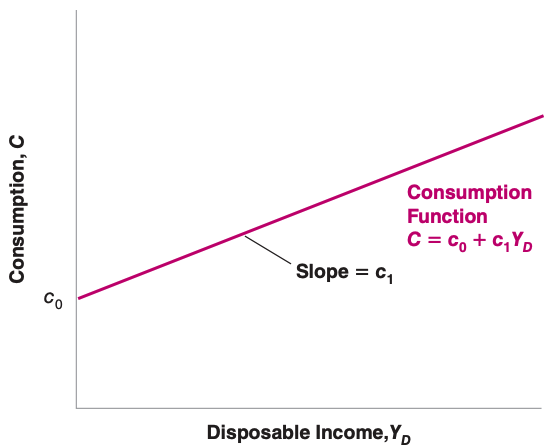
\includegraphics[scale=0.4]{images/03-c-yd.png}
    \end{center}

    {\bf disposable income }$Y_D$, is given by 
    $$Y_D\equiv Y-T$$
    where $Y$ is {\bf income } and $T$ is taxes paid minus government 
    transfers received by consumers(e.g. Medicare).

    Then we will have: 
    $$C=c_0+c_1(Y-T)$$

    Hence higher income increases consumption, while higher taxes 
    decrease consumption.



    \subsection{Investment($I$)}

    Instead of {\bf endogenous}(variables that depend on other variables)
    like the consumption above, {\bf investment} is not explained within 
    the model and is taken {\it as given}, which is called {\bf exogenous.}
    $$I=\overline{I}$$
    Here we put a bar to remind us we take investment as given.

    We take investment as given to keep our model simple. 
    But the assumption is not accurate in reality.

    \subsection{Government Spending($G$)}

    $T$(taxes minus government transfers) and $G$ 
    describe {\bf fiscal policy} — the choice of taxes and spending by the 
    government. We will take G and T as {\bf exogenous}, but the reason is 
    different from investment: 
    \begin{enumerate}
        \item governments do not behave with the same {\bf regularity} as consumers 
        or firms, so there is no reliable rule
        \item more importantly, one of the tasks of macroeconomic is to think 
        about the implications of alternative spending and tax decisions. 
        We want be able to say, ``{\it if the government were to choose these 
        values for $G$ and $T$, ... would happen.}''
    \end{enumerate}

    \section{The Determination of Equilibrium Output}

    Still, we assume a closed economy where exports and imports are both 0. 
    Then,
    $$Z\equiv C+I+G$$
    $$Z=c_0+c_1(Y-T)+\overline{I}+G$$

    Moreover, if we assume firms {\bf do not hold inventories}, in which case 
    {\bf inventory investment} is always 0. Then {\bf equilibrium in the good 
    market} requires the production $Y$ be equal to the demand for goods $Z$: 
    $$Y=Z$$
    This is called an {\bf equilibrium condition}, and replace demand $Z$, 
    $$Y=c_0+c_1(Y-T)+\overline{I}+G$$

    \textit{ \textbf{Remark}: production, $Y$(the left side) is equal to demand(the right
    side). Demand in turn depends on income $Y$, which is equal to production. }

    {\bf Models} include three types of equations: 
    {\bf identities, behavioral equations, and equilibrium conditions.} 
    We now have seen examples of each: The equation defining disposable income 
    is an {\bf identity}, the consumption function is a {\bf behavioral equation}, 
    and the condition that production equals demand is an {\bf equilibrium condition}.


    {\it This is the end of lecture note. Last modified: Sep 15.\\
    Sep 15: Add details during class.}

\end{spacing}
\end{document}
